\chapter{Implementation}

\tcol[gray]{\section{Betraktninger:}}
\besk{"Det man har utviklet" — Kyrre}
\besk{"Det er her man henter fisken tilbake på land (blant andre steder — som f.eks. der man dokumenterer eksperimentene sine godt)."ish — Jim}

\gjor{Skriv opp Worklog-materiale dandert i henhold til gode master-theses}

\gjor{
	\textbf{Svar på disse spørsmålene (kompilert fra Tønnes sin masteroppgave):}
	What does the chapter do? What's the main goal of the design/implementation/developed system? What do these goals require? Why did you make the design-choices you made? What advantages do these choices ensure/enable? Give a short chapter-outline (perhaps first about the design, my additional Self-Awareness component, manual choice of initial parameters, and then the benchmark or målestokk or performance measure I use to evaluate with).
}

\gjor{Se på Tønnes sin Masteroppgave og 'Archive History'-kommentarene nederst i .tex-fila for inspirasjon}

\newpage


% Implementation-introtekst
This chapter gives an overview of the developed multi-robot system. The main goal of the implemented system is to allow for a multi-robot (musical) collective to interact with each other in order to achieve emergent and co-ordinating/co-operative behaviour—synchronization specifically in our case—with varying degrees of difficulty and certainty in the environment and communication. More specifically, the goal with the design is to enable the robot collective to achieve so-called \textit{harmonic synchronization} within a relatively short time, much depending on the design parameters and environment conditions. What's meant by \textit{harmonic synchronization} will be expounded on in \tcol{subseksjon X}. These goals firstly require the modelling of oscillators with their properties, like phase and frequency. To allow for interaction and communication between the agents, mechanisms so that the agents can transmit "fire"-signals, as well as listen for other agents's "fire"-signals, is necessary as well.



% Seksjon om baselinen (Nymoens ideer og algoritmer implementert i mitt system i Unity).
\section{The baseline: The musical multi-robot system}
\besk{Nymoens ideer og algoritmer implementert i mitt system i Unity}

Envision that we have a multi-agent collective scenario consisting of musical robots, modelled as oscillators, solely communicating through audio-signals, entraining to synchronize to each other by adjusting their phases and frequencies when or after hearing each other's audio-signals. These audio-signals, also referred to as "fire"-signals, are transmitted when an agent's oscillator \textit{peaks} (i.e. having phase $\phi(t)=1$). All agents have the ability to listen for such transmitted "fire"-signals from their neighbours, which they then will use as a trigger to adjust themselves according to some well-designed update-functions.

% First figure to get a quick idea of what the system does:
% MÅ FIKSE ELLER FJERNE!!!!!:
% - Fjern den Gule/Orange Dr. Squiggle'n fra Spawne-lista (pga. tvetydighet pga. gul fire-color).
% - Få god oppløsning og kanskje bruke .PNG istedenfor .JPG.
% - Ikke skape misoppfatningen om at alle agenter må fyre samtidig for å være *harmonisk* synkroniserte.
% + SKAL JEG KANSKJE BARE DROPPE HELE DENNE FIGUREN SIDEN DEN PÅ EN MÅTE BARE GJØR DETTE?
\begin{figure}[h] % Intro-illustration for a quick and easy way to get an idea of my design.
	\centering
		\begin{subfigure}[t]{.5\textwidth}
			\centering\captionsetup{width=.9\linewidth}%
			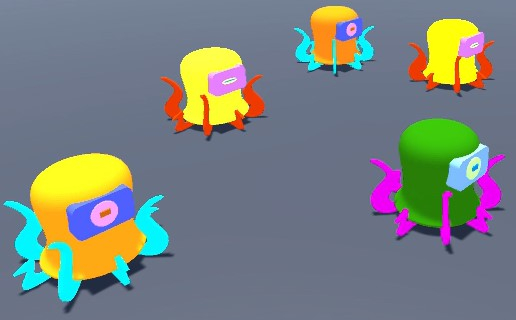
\includegraphics[width=0.9\linewidth]{Assets/Figures/IntroUnsynch.jpg}
			\caption{The agents firing asynchronously at first. Here, only the two Dr. Squiggles with red tentacles are firing simultaneously, but the rest are not.}
			\label{initial:unsynch}
		\end{subfigure}%
		\begin{subfigure}[t]{.5\textwidth}
			\centering\captionsetup{width=.9\linewidth}%
			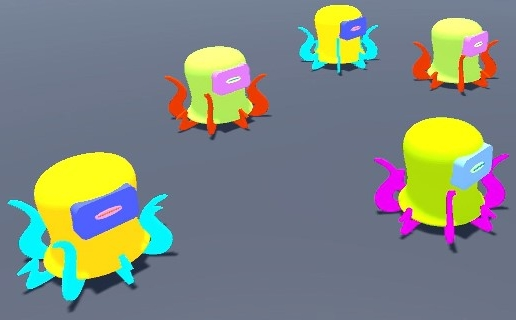
\includegraphics[width=0.9\linewidth]{Assets/Figures/IntroSynch.jpg}
			\caption{Seconds later, after having listened to each other's fire-event signals and adapted themselves accordingly, the agents are here firing synchronously.}
			\label{initial:synch}
		\end{subfigure}
	\caption{Synchronization (of phases) in a musical robot collective achieved. \tcol{(NB! Dette skaper kanskje en misoppfatning om at alle noder må fyre samtidig for å være synkroniserte.. Husk at dette ikke er tilfellet med \textit{harmonisk synkronisering})}}	% Gammel caption: "The musical agents, also known as M. J. Krzyzaniak's Dr. Squiggles, are actively listening for signals from each other's fire-events, entraining to synchronize to each other accordingly." Cite Pierre her?
	\label{initial}
\end{figure}


% Subseksjon om den enkelte noden/agenten med alle egenskaper den har osv. (som f.eks. en oscillator-komponent (jf. Nymoens Implementation-seksjon))
\subsection{The node: the musical robot individual}
\besk{Subseksjon om den enkelte noden/agenten med alle egenskaper den har osv. (som f.eks. en oscillator-komponent (jf. Nymoens Implementation-seksjon))}

% Subseksjon om kommunikasjonsmetoden til agentene: audio-/"fire"-signalet
\subsection{Robot communication: the "fire"-signal}
\besk{Subseksjon om kommunikasjonsmetoden til agentene: audio-/"fire"-signalet}

% Subseksjon om target-staten til systemet: harmonisk synkroni
\subsection{System target state: Harmonic Synchrony}
\besk{Subseksjon om target-staten til systemet: harmonisk synkroni}

The goal and target state of the system is \textit{harmonic synchrony}, as K. Nymoen et al. \cite{nymoen_synch} coined it when ...



% Seksjon om mitt bidrag (skill tydelig på mine bidrag og de jeg ikke har gjort noe med)

\section{The new proposed algorithm: an additional Self-Awareness component}









% Archive History:

	% \section{Benchmark}
		% \besk{Her jeg beskriver Nymoens algoritmer og formler (originalt), men \opphoy{sånn jeg har implementert det i Unity}}
	
		% \gjor{Vurder om 'Benchmark' bør deles opp i sin egen sub-seksjon i det hele tatt — eller f.eks. slås sammen med 'Proposed Algorithm'}
	
		% \besk{(Hentet fra Samuelsens master?) Presentering av metoden brukt til å evaluere ytelsen av den foreslåtte/proposed'e algoritmen. Først er kanskje en referanse-algoritme brukt for sammenlikning beskrevet. Deretter er (f.eks. objektiv-) funksjoner brukt i testene forklart. Endelig (til slutt) er kanskje miljøene/environments'a og parameterne brukt presentert}
		
		
	% \section{Proposed Algorithm}
		% \besk{Evt. her jeg skriver om Self-Awareness-komponenten(e) jeg legger til ang. Belief-awareness og/eller Expectation-awareness (jf. det jeg og Kyrre snakka om Mid-November på 'reMarkable -> Møter -> ROBIN -> Kyrre')}
	
		% \gjor{Vurder om 'Proposed Algorithm' bør deles opp i sin egen sub-seksjon i det hele tatt — eller f.eks. slås sammen med 'Benchmark'}
	